\documentclass{report}
\usepackage{amsmath, amssymb, amsthm}
\usepackage{geometry}
\geometry{a4paper, margin=0.8in}
\usepackage{float}
\usepackage{tikz}
\usetikzlibrary{calc, decorations.pathreplacing}
\usepackage{pgfplots}
\pgfplotsset{compat=1.18}
\usepackage{xcolor}
\usepackage{tcolorbox}
\tcbuselibrary{theorems}
\usepackage{eurosym}
\usepackage{fancyhdr}
\usepackage{booktabs}
\usepackage{listings}

\lstdefinestyle{tcblatex}{
    language=[Visual]Basic,
    basicstyle=\ttfamily\footnotesize,
    keywordstyle=\bfseries,
    commentstyle=\itshape,
    stringstyle=\ttfamily,
    showstringspaces=false,
    breaklines=true,
    columns=fullflexible
}

\begin{document}

\pagestyle{fancy}
\fancyhf{}
\rhead{Report 3 \;|\; Stochastic Methods for Finance \;|\; \thepage}
\renewcommand{\headrulewidth}{0.4pt}
\setlength{\headheight}{14pt}
\thispagestyle{plain} 

% --- HEADER PROFESSIONALE ---
\begin{flushleft}
    {\large \textbf{Stochastic Methods for Finance - Report 3}} \\
    \rule{\textwidth}{0.4pt} \\ 
    \textbf{Author:} Davide Quartucci \hfill \textbf{Date:} March 30, 2026 \\
\end{flushleft}

\begin{center}
    \fcolorbox{black}{gray!10}{
        \begin{minipage}{0.95\textwidth}
            \small \textit{Every step implementation can be checked in the provided file:} \texttt{Report3\_Quartucci\_Davide.xlsm}
        \end{minipage}
    }
\end{center}

\section{Introduction}
In this report, we analyze the pricing of a European Call option to compare how fast two different binomial models converge to the exact price. We look at the standard Cox-Ross-Rubinstein (CRR) model and the Leisen-Reimer (LR) model, using the closed-form Black-Scholes (B\&S) price as our true benchmark. The parameters for our option are: Spot Price $S=100$, Strike Price $K=100$, Maturity $T=1$ year, Risk-free rate $r=1\%$, and Volatility $\sigma=20\%$.

\section{VBA Implementation and Excel Setup}
We implemented the models using custom VBA scripts so we could easily test them across many different time steps without overloading the spreadsheet. We built three main functions:
\begin{itemize}
    \item \texttt{BS\_Call}: Gives us the exact benchmark price (8.4333).
    \item \texttt{Binomial\_CRR\_Call}: Runs the standard CRR tree.
    \item \texttt{Binomial\_LR\_Call}: Runs the LR tree using the Peizer-Pratt inversion to place the nodes.
\end{itemize}

In Excel, we set up two main simulation tables. The first one tests $n$ from 10 to 100 (in steps of 5) to see what happens when we alternate between even and odd steps. The second table only looks at odd steps (from 11 to 191) so we can observe the LR model working under its optimal conditions.

\section{Price Convergence Analysis}
Here we compare how the CRR and LR prices approach the Black-Scholes benchmark, looking first at the plotted trajectories and then at the math behind the trees.

\subsection{The Even/Odd Effect and LR Instability}
Figure \ref{fig:price_even_odd} shows a clear difference between the models when we include both even and odd values of $n$. The CRR price does its usual "zig-zag" around the Black-Scholes value, slowly getting closer as $n$ increases. The LR model, on the other hand, goes completely off the rails for even steps, showing massive pricing errors.

\begin{figure}[H]
    \centering
    
\includegraphics[width=0.8\textwidth]{Picture1.png}
    \caption{Price Convergence: Even/Odd Steps. The CRR model shows its typical zig-zag, while the LR model is highly unstable on even steps.}
    \label{fig:price_even_odd}
\end{figure}

The reason for this lies in the geometry of the tree. The LR model relies on the Peizer-Pratt inversion to perfectly center the tree around the strike $K$. This works beautifully for odd $n$, but for even $n$, the centering breaks down and messes up the probabilities.

\subsection{Convergence on Odd Steps}
When we filter the data and only look at odd steps (Figure \ref{fig:price_odd}), the LR model really shines. It approaches the Black-Scholes value rapidly and smoothly, without any oscillations, while the CRR model still converges much more slowly.

\begin{figure}[H]
    \centering
    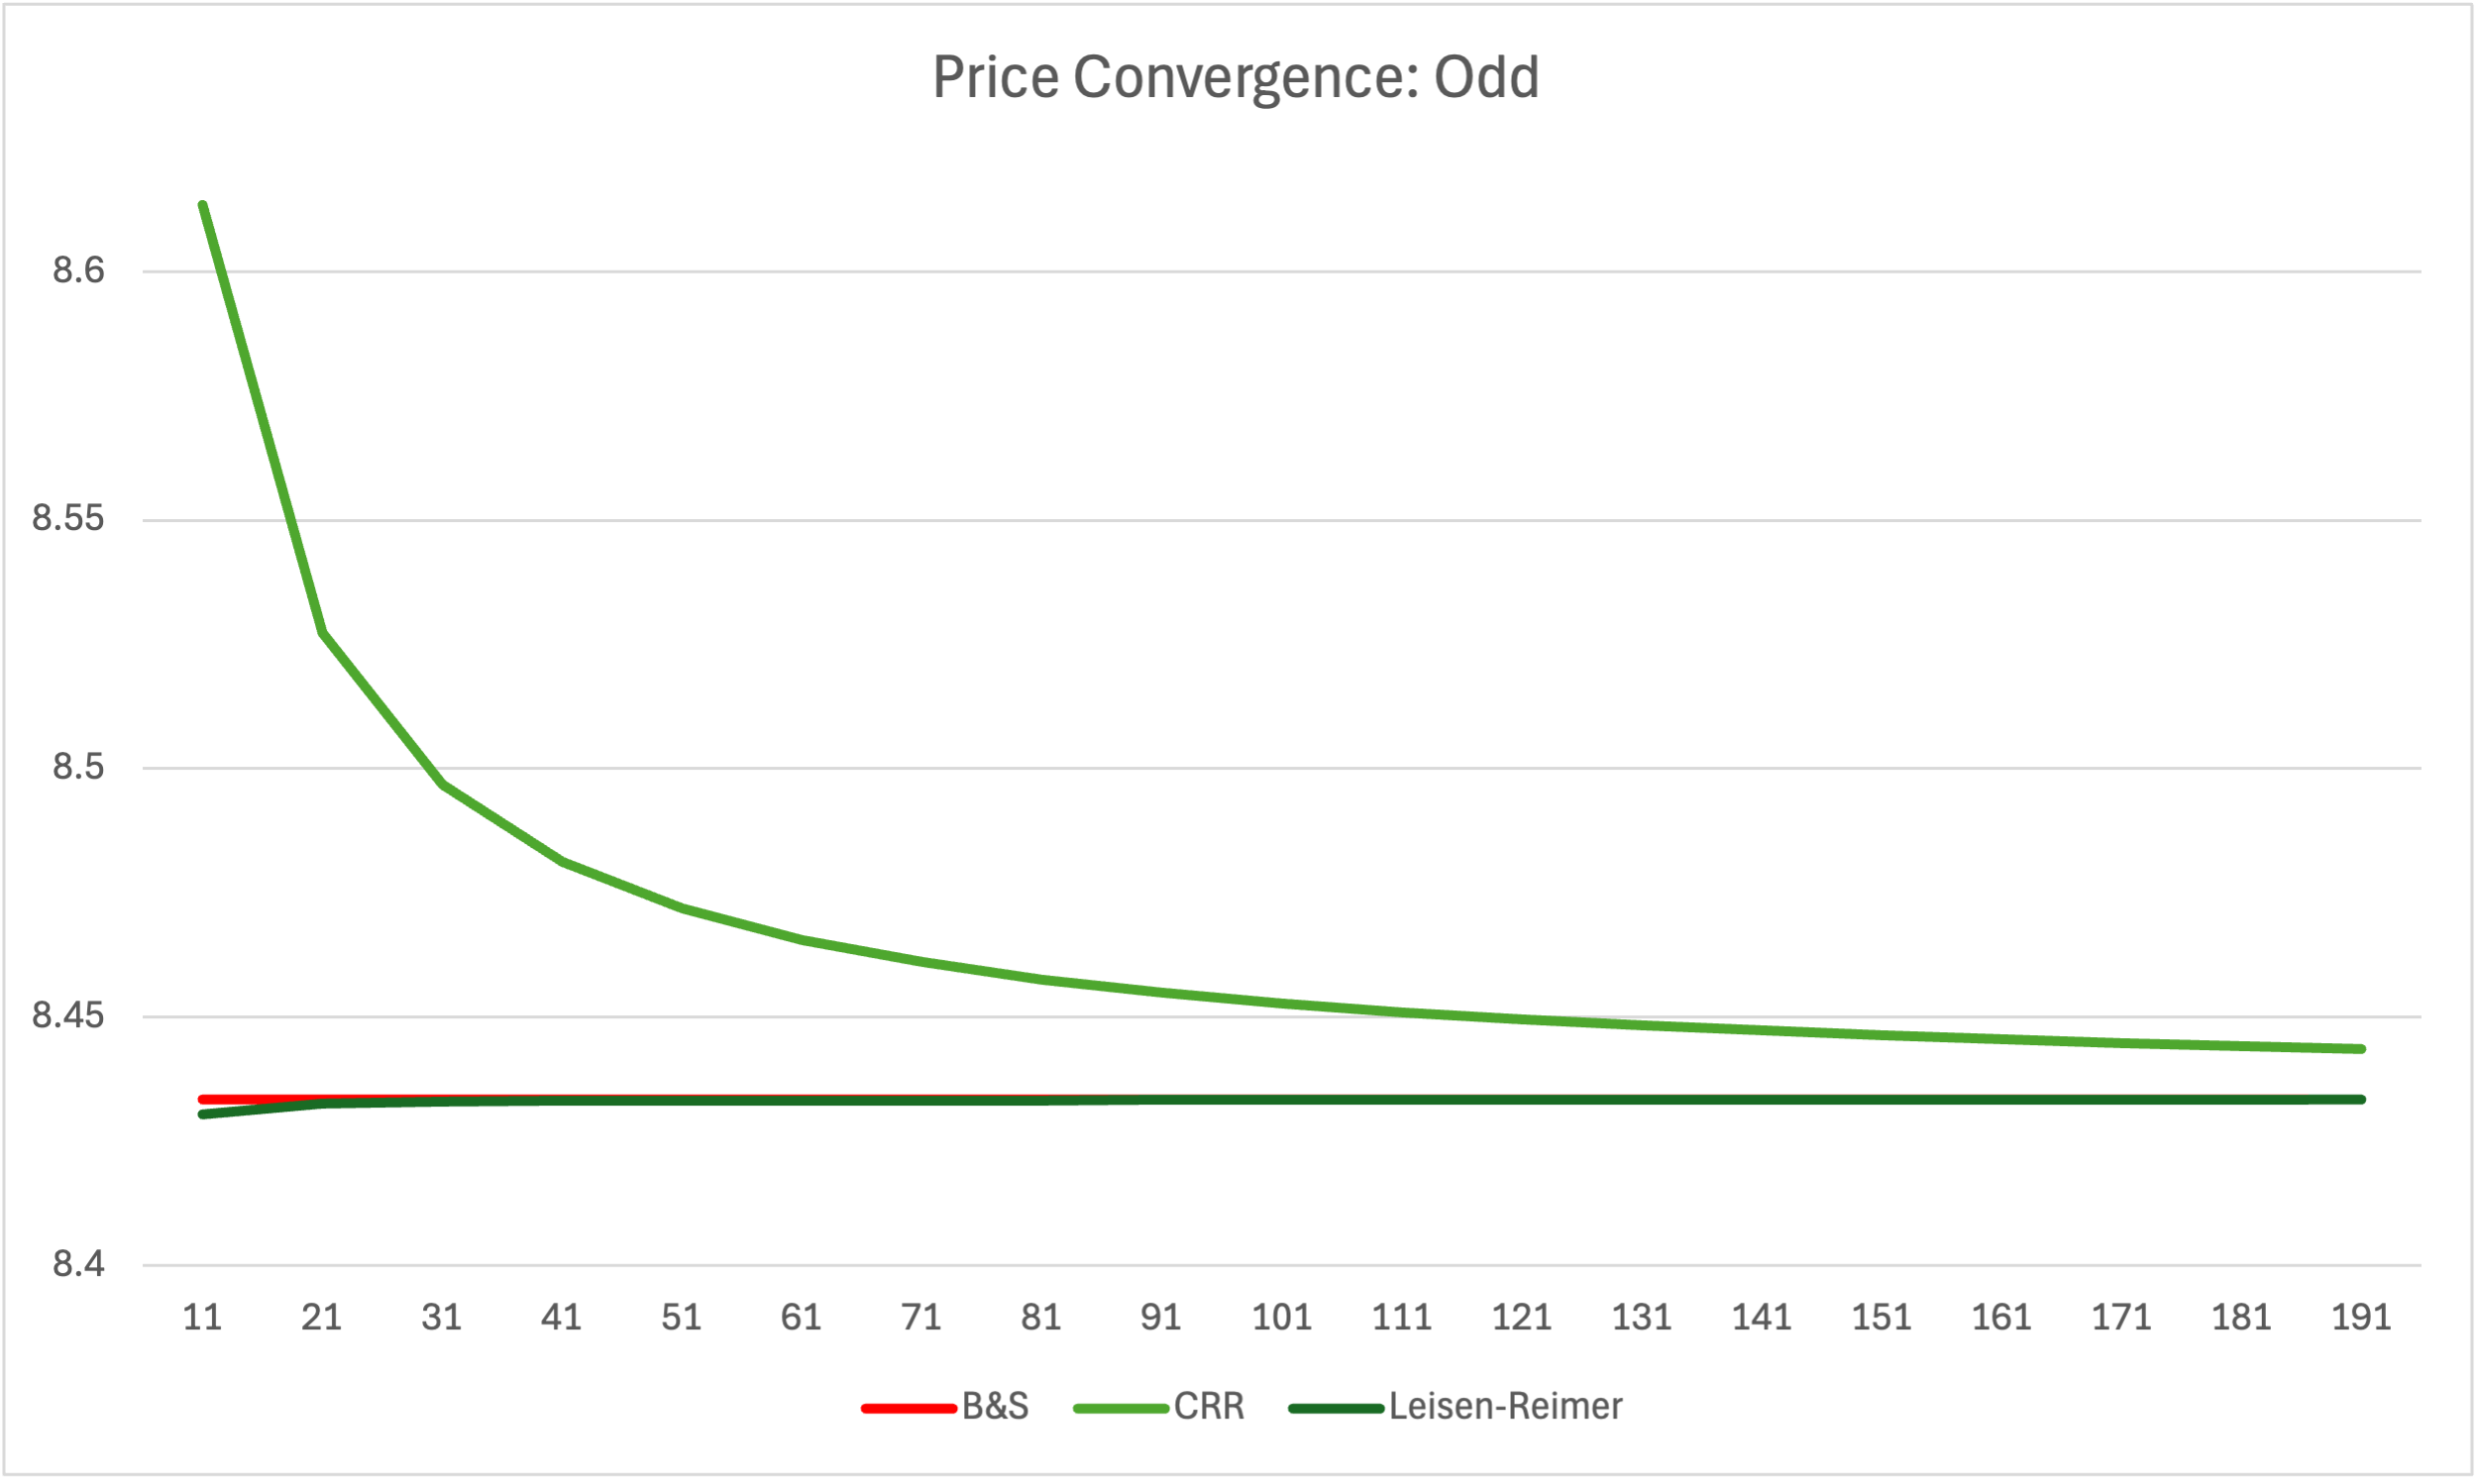
\includegraphics[width=0.8\textwidth]{Picture2.png}
    \caption{Price Convergence: Odd Steps Only. The LR model quickly aligns with the exact Black-Scholes price.}
    \label{fig:price_odd}
\end{figure}

\subsection{Theoretical Justification: Tree Geometry}
The contrast between the two models happens because of how they position their terminal nodes relative to the strike $K$.

\textbf{The CRR Model} \\
CRR builds the tree using jump factors that depend only on volatility and time:
$$u = e^{\sigma \sqrt{\Delta t}} \quad \text{and} \quad d = e^{-\sigma \sqrt{\Delta t}}$$
Because $K$ isn't part of this formula, the terminal nodes don't align perfectly with the strike. As $n$ changes, the grid shifts back and forth around $K$, which causes that annoying $\mathcal{O}(1/n)$ zig-zag effect.

\textbf{The LR Model} \\
Leisen and Reimer use the \textbf{Peizer-Pratt inversion} to force the terminal nodes to center perfectly around $K$. This is what gives the model its speed, but it also explains the odd/even issue:
\begin{itemize}
    \item \textbf{Odd $n$:} the terminal layer has an even number of nodes ($n+1$). This creates a perfectly symmetric gap in the middle where $K$ fits flawlessly. The model is stable and hits its $\mathcal{O}(1/n^2)$ convergence.
    \item \textbf{Even $n$:} the terminal layer has an odd number of nodes, meaning there's one node right in the middle. Forcing the continuous distribution to center on this single node distorts the parameters and causes the large errors we saw in the first graph.
\end{itemize}

\section{Investigation of Convergence Rates}
To find the actual rate of convergence, we plotted the absolute error on a Log-Log scale. On this kind of chart, an error function like $E = c \cdot n^k$ turns into a straight line, and the slope $k$ is our rate of convergence.

First, we plotted the errors for all steps (Figure \ref{fig:error_even_odd}). As you can see, the LR model's instability on even steps creates huge spikes. Trying to fit a trendline through this noisy data wouldn't give us a reliable convergence rate. This visually proves why we need to leave the even steps aside.

\begin{figure}[H]
    \centering
    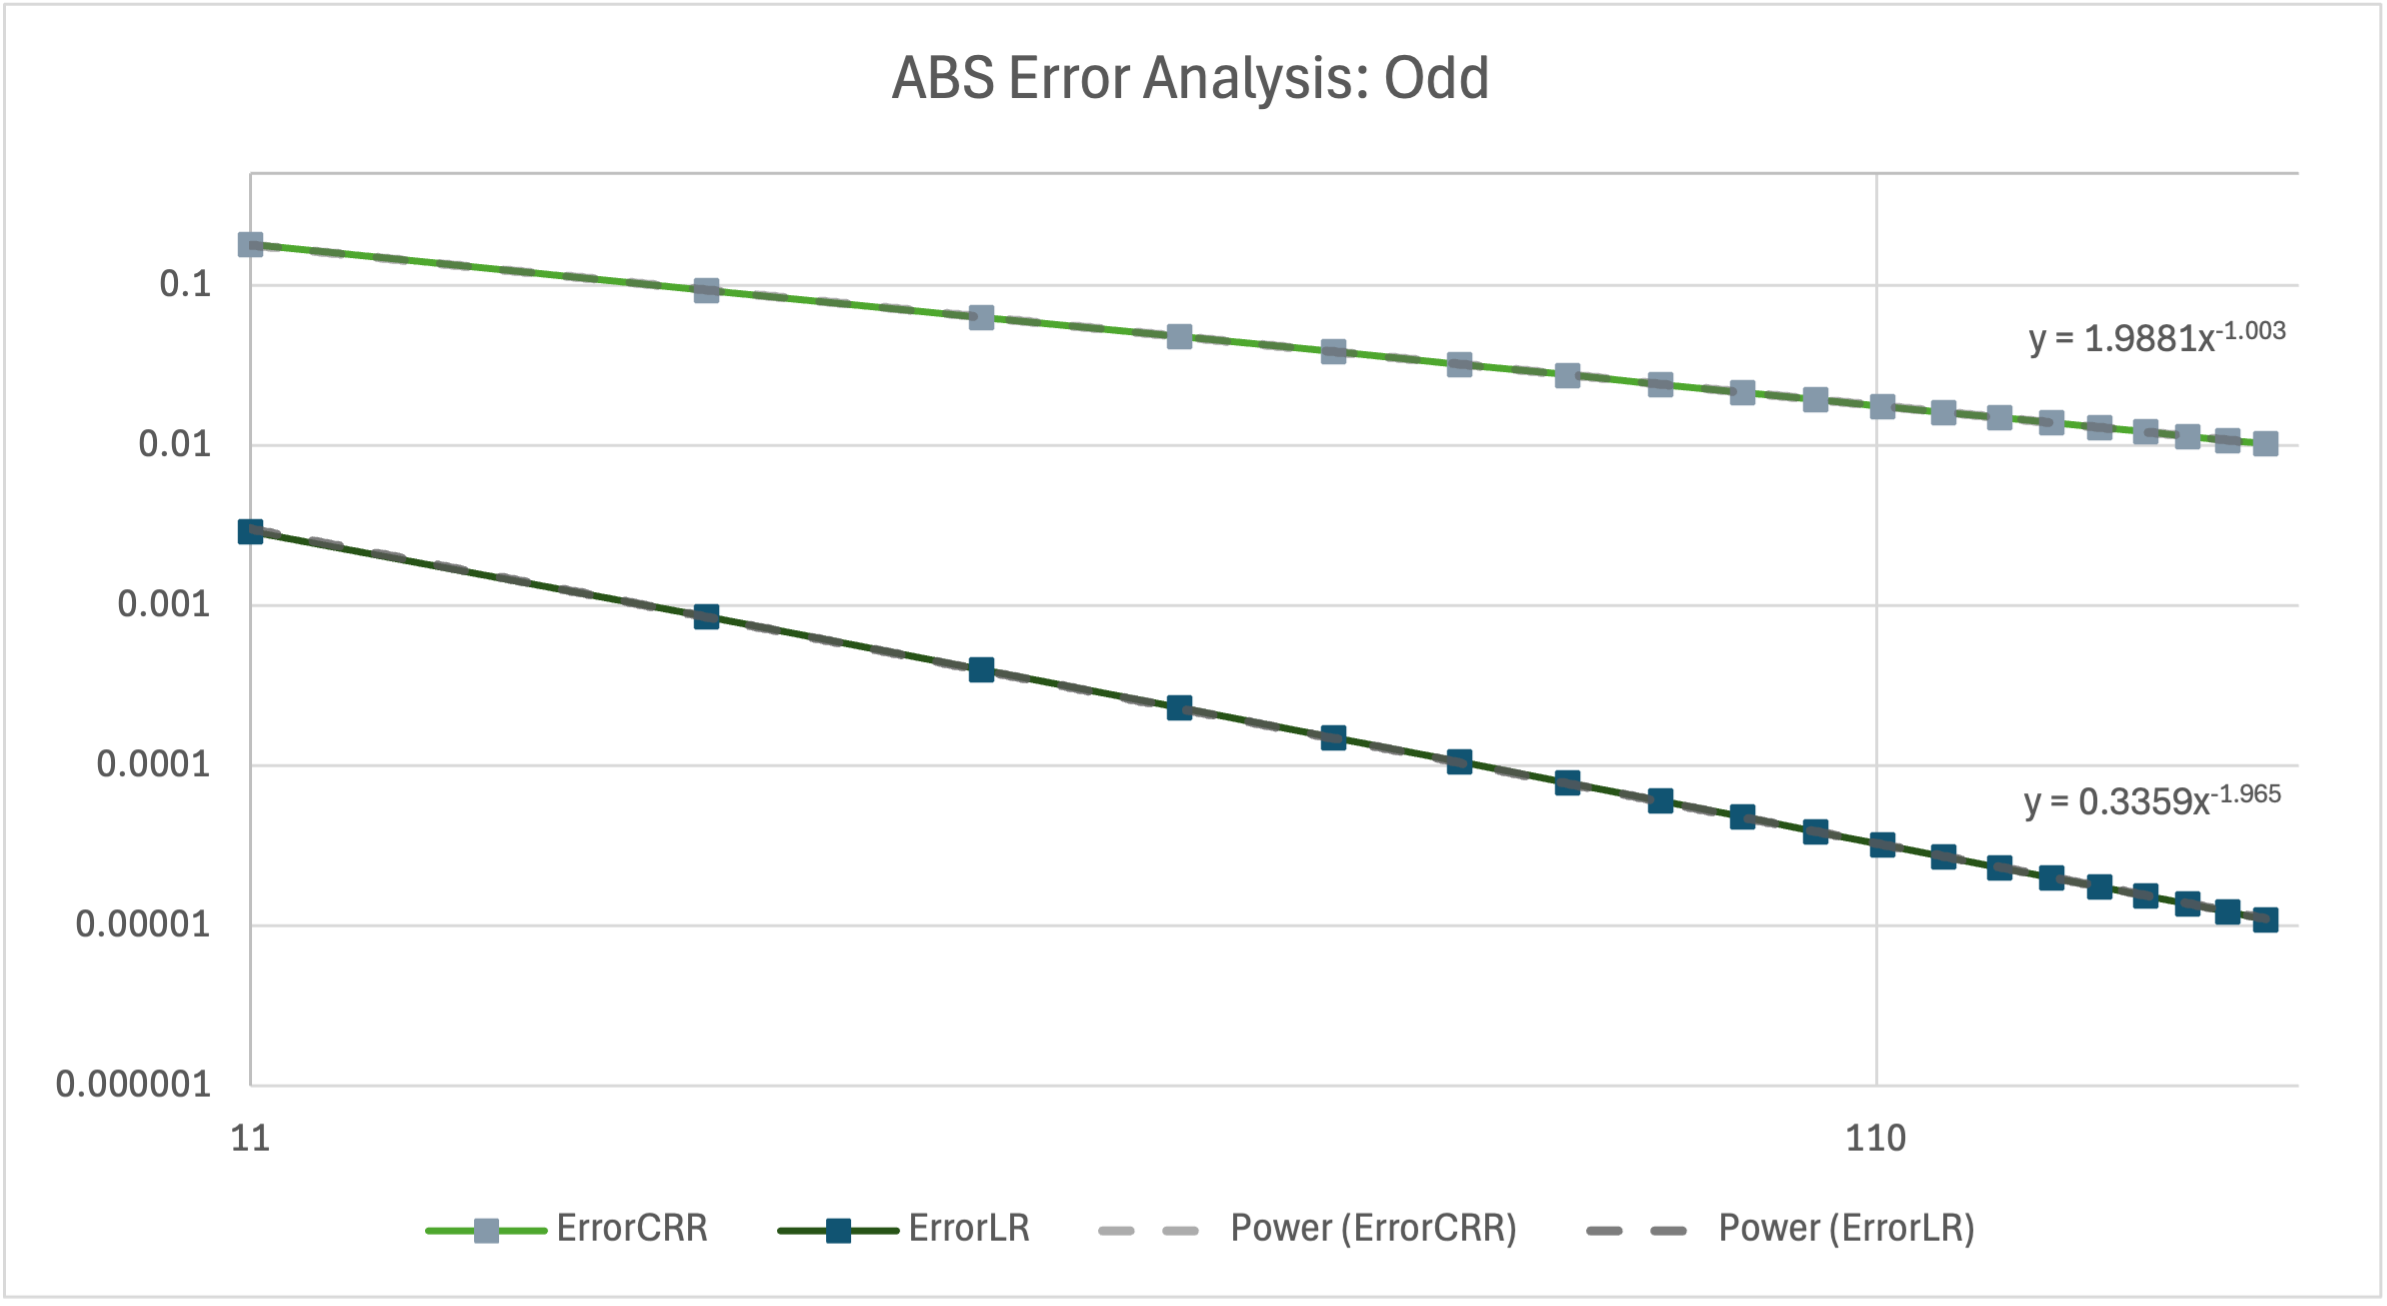
\includegraphics[width=0.8\textwidth]{Picture3.png} % Assicurati che questo sia il grafico Errori Pari/Dispari
    \caption{Absolute Error Convergence: Even/Odd Steps. The massive spikes in the LR model make it impossible to extract a clean trendline.}
    \label{fig:error_even_odd}
\end{figure}

Once we filter for only the odd steps (Figure \ref{fig:error_odd}), the data points form clean straight lines. To extract the exact rates, we didn't just calculate them step-by-step, because the discrete nature of the tree would still create too much local noise. Instead, just like we did in our previous report, we used an Ordinary Least Squares (OLS) regression on the whole dataset. This gives us the true global trend as $n \to \infty$.

Table \ref{tab:rates_summary} compares our theoretical expectations with the empirical rates we extracted, which match the equations shown in Figure \ref{fig:error_odd}.

\begin{table}[H]
    \centering
    \renewcommand{\arraystretch}{1.3}
    \begin{tabular}{|l|c|c|}
        \hline
        \textbf{Pricing Model} & \textbf{Theoretical Convergence} & \textbf{Empirical Rate ($k$)} \\
        \hline
        CRR (Standard Binomial) & $\mathcal{O}(1/n)$ (Expected: $-1$) & $-1.00$ \\
        Leisen-Reimer (Odd Steps) & $\mathcal{O}(1/n^2)$ (Expected: $-2$) & $-1.96$ \\
        \hline
    \end{tabular}
    \caption{Summary of theoretical versus empirically calculated convergence rates.}
    \label{tab:rates_summary}
\end{table}

\begin{figure}[H]
    \centering
    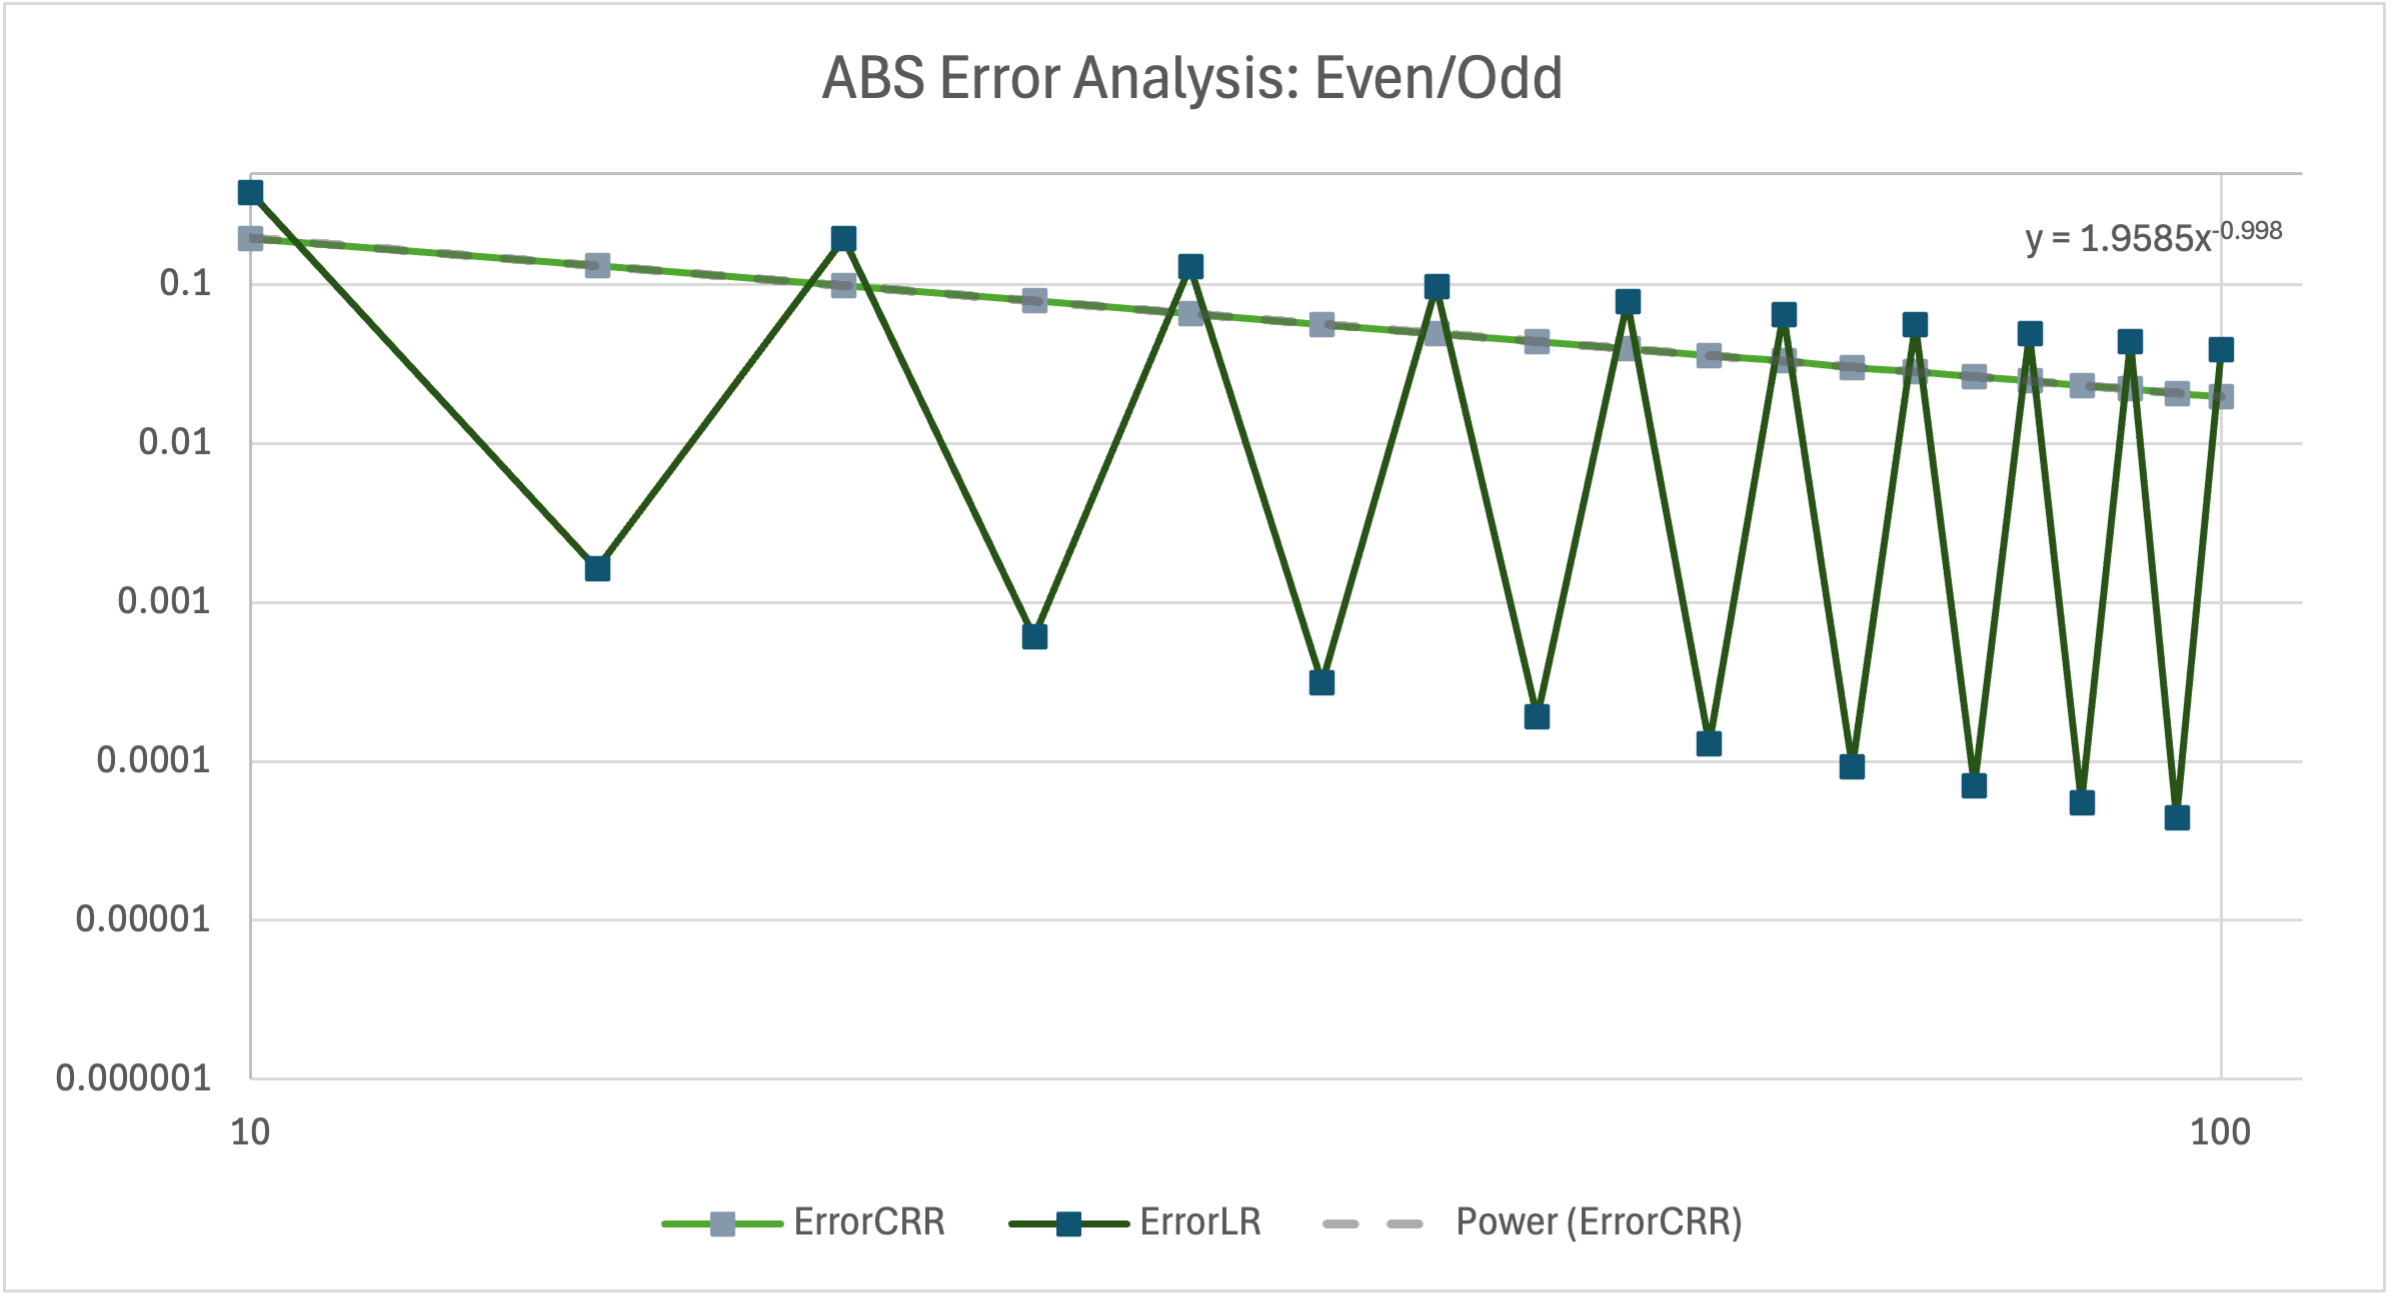
\includegraphics[width=0.8\textwidth]{Picture4.png} % Assicurati che questo sia il grafico Errori SOLO Dispari
    \caption{Absolute Error Convergence: Odd Steps Only. The OLS trendlines clearly reveal the convergence rates.}
    \label{fig:error_odd}
\end{figure}

Looking at the results:
\begin{itemize}
    \item \textbf{CRR Model}: The trendline slope is $-1.00$, confirming the slow $\mathcal{O}(1/n)$ convergence.
    \item \textbf{LR Model}: The slope for the odd data is $-1.96$. This validates the theory, proving that the LR model actually achieves a quadratic convergence rate of $\mathcal{O}(1/n^2)$.
\end{itemize}

\section{Conclusion}
In conclusion, our analysis shows that while the standard CRR model is a reliable starting point, it converges quite slowly and suffers from a persistent zig-zag effect. The Leisen-Reimer model fixes this by cleverly centering the tree on the strike price, but with a major catch: we must strictly use an odd number of steps to avoid severe geometric instability.

By running an OLS power regression on the errors, we managed to empirically validate the theory. The extracted rates ($-1.00$ for CRR and $-1.96$ for LR) show that the LR model successfully accelerates convergence from $\mathcal{O}(1/n)$ to $\mathcal{O}(1/n^2)$. As long as we stick to odd steps, it is a much faster and more efficient tool for pricing options.

\begin{lstlisting}[style=tcblatex, title={VBA Code Snippet}]
' ==============================================================================
' Based on standard Black-Scholes continuous pricing formula.
' Calculates the theoretical price of a European Call option.
' ==============================================================================
Function BS_Call(S As Double, K As Double, T As Double, r As Double, vol As Double) As Double
    Dim d1 As Double, d2 As Double
    Dim Nd1 As Double, Nd2 As Double
    
    ' Handle the expiration case (T=0)
    If T <= 0 Then
        BS_Call = Application.Max(S - K, 0)
        Exit Function
    End If
    
    ' Calculate d1 and d2 parameters
    d1 = (Log(S / K) + (r + 0.5 * vol ^ 2) * T) / (vol * Sqr(T))
    d2 = d1 - vol * Sqr(T)
    
    ' Calculate the Cumulative Standard Normal Distribution using Excel's built-in function
    Nd1 = Application.WorksheetFunction.Norm_S_Dist(d1, True)
    Nd2 = Application.WorksheetFunction.Norm_S_Dist(d2, True)
    
    ' Calculate final Call price
    BS_Call = S * Nd1 - K * Exp(-r * T) * Nd2
End Function


' ==============================================================================
' Based on the standard Cox-Ross-Rubinstein (1979) model.
' Prices a European Call using the standard binomial tree method.
' ==============================================================================
Function Binomial_CRR_Call(S As Double, K As Double, T As Double, r As Double, vol As Double, n As Integer) As Double
    Dim dt As Double, u As Double, d As Double, p As Double
    Dim i As Integer, j As Integer
    Dim V() As Double
    
    ' Calculate CRR parameters
    dt = T / n
    u = Exp(vol * Sqr(dt))
    d = 1 / u
    p = (Exp(r * dt) - d) / (u - d)
    
    ' Create an array for the terminal nodes
    ReDim V(0 To n)
    
    ' Step 1: Calculate the Payoff at expiration (leaf nodes)
    For i = 0 To n
        V(i) = Application.Max(S * (u ^ (n - i)) * (d ^ i) - K, 0)
    Next i
    
    ' Step 2: Backward induction (calculating back to the initial node)
    For j = n - 1 To 0 Step -1
        For i = 0 To j
            V(i) = Exp(-r * dt) * (p * V(i) + (1 - p) * V(i + 1))
        Next i
    Next j
    
    Binomial_CRR_Call = V(0)
End Function


' ==============================================================================
' Based on formulas from the paper:
' "Binomial Models for Option Valuation - Examining and Improving Convergence"
' by Dietmar Leisen & Mark Reimer (1995).
' Peizer-Pratt inversion helper function and the LR Binomial Model.
' ==============================================================================

' Helper function for the Peizer-Pratt approximation used in the L-R paper
Function Peizer_Pratt(z As Double, n As Integer) As Double
    Dim temp As Double
    temp = (z / (n + 1 / 3 + 0.1 / (n + 1))) ^ 2 * (n + 1 / 6)
    Peizer_Pratt = 0.5 + Sgn(z) * 0.5 * Sqr(1 - Exp(-temp))
End Function

' Main Leisen-Reimer pricing function
Function Binomial_LR_Call(S As Double, K As Double, T As Double, r As Double, vol As Double, n As Integer) As Double
    Dim dt As Double
    Dim d1 As Double, d2 As Double
    Dim p As Double, p_prime As Double
    Dim u As Double, d As Double
    Dim i As Integer, j As Integer
    Dim V() As Double
    
    dt = T / n
    
    ' Black-Scholes d1 and d2 parameters
    d1 = (Log(S / K) + (r + 0.5 * vol ^ 2) * T) / (vol * Sqr(T))
    d2 = d1 - vol * Sqr(T)
    
    ' Modified Leisen-Reimer probabilities using Peizer-Pratt
    p_prime = Peizer_Pratt(d1, n)
    p = Peizer_Pratt(d2, n)
    
    ' Calculate up and down factors forcing convergence around the strike
    u = Exp(r * dt) * p_prime / p
    d = (Exp(r * dt) - p * u) / (1 - p)
    
    ReDim V(0 To n)
    
    ' Step 1: Payoff at expiration
    For i = 0 To n
        V(i) = Application.Max(S * (u ^ (n - i)) * (d ^ i) - K, 0)
    Next i
    
    ' Step 2: Backward induction
    For j = n - 1 To 0 Step -1
        For i = 0 To j
            V(i) = Exp(-r * dt) * (p * V(i) + (1 - p) * V(i + 1))
        Next i
    Next j
    
    Binomial_LR_Call = V(0)
End Function
\end{lstlisting}

\end{document}